\documentclass{beamer}
\usepackage[orientation=portrait, size=a0, scale=1]{beamerposter}
\usepackage{multicol} % This is so we can have multiple columns of text side-by-side
\usepackage{parskip}
%\usepackage{enumitem}
%\setlist[itemize]{parsep=0pt}
%\setlist[enumerate]{parsep=0pt}
%\parindent=0em

%% Bibliography stuff (biblatex):
\usepackage[
backend=bibtex,
firstinits=true, 
isbn=false, 
url=false,
maxbibnames=3,
doi=false,
clearlang=true,
terseinits=true,
citestyle=numeric,
autolang=hyphen,
clearlang=true
]{biblatex} 

\AtEveryBibitem{%
  \clearlist{language}%
}


\renewcommand*{\bibfont}{\small}
\bibliography{library.bib}


\usetheme{BCCRC}
%\usetheme{Madrid}
\setbeamerfont{frametitle}{size={\fontsize{200}{36}}}


\title{Screw: tools for building reproducible \\ single-cell epigenomics workflows}
\author{Kieran O'Neill\textsuperscript{1}, Chelsey Fang\textsuperscript{1}, Benjamin Decato\textsuperscript{2}, Azhar Khandekar\textsuperscript{3}, Alexander Goncearenco\textsuperscript{3}, Ben Busby\textsuperscript{3} , Aly Karsan\textsuperscript{1}}


\institute{\textsuperscript{1} Genome Sciences Centre, BC Cancer Agency, Vancouver, BC, Canada \textsuperscript{2} Molecular \& Computational Biology Department, University of Southern California, Los Angeles, California, USA \textsuperscript{3} National Center for Biotechnology Information, National Institutes of Health, Bethesda, Maryland, USA}

\begin{document}
\begin{frame}[t, squeeze, fragile]
\begin{columns}[t]

%%%%%%%%%%%%%%%%%%%%%%%%%%%%%%%%%%%%%%%%%%%%%%%%%%%%%%%%%%%%%%%%%%%%%%%%%%%%%%%%%%%%
% COLUMN 1
%%%%%%%%%%%%%%%%%%%%%%%%%%%%%%%%%%%%%%%%%%%%%%%%%%%%%%%%%%%%%%%%%%%%%%%%%%%%%%%%%%%%


\begin{column}{.32\textwidth}


\begin{block}{Background: Single-cell DNA Methylation Sequencing}
DNA methylation is a heritable epigenetic mark that shows a strong correlation with transcriptional activity. 
The gold standard for detecting DNA methylation is whole genome bisulfite sequencing (WGBS). 
Recently, WGBS has been performed successfully on single cells (SC-WGBS) \cite{Schwartzman2015}.
The resulting data represents a fundamental shift in the capacity to measure and interpret DNA methylation, especially in rare cell types and contexts where subtle cell-to-cell heterogeneity is crucial, such as in stem cells or cancer. 
However, although some software tools have been published, and several existing studies have tended to use similar methods, no standardized pipeline for the analysis of SC-WGBS yet exists.



\begin{figure}
\begin{center}
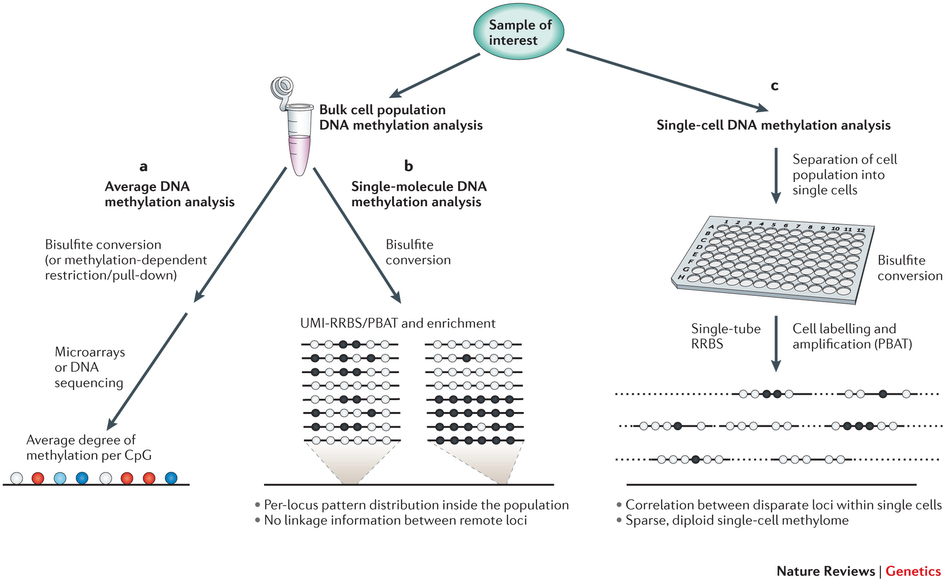
\includegraphics[width=0.9\textwidth]{figures/nrg3980-f1.jpg}
\end{center}
\caption[]{\textbf{DNA Methylation, both bulk and single cell}
Schwartzman et al (2015) Nature Reviews in Genetics (used by permission) }
\end{figure}

\end{block}

\begin{block}{Screw: Single Cell Reproducible Epigenomics Workflow}
%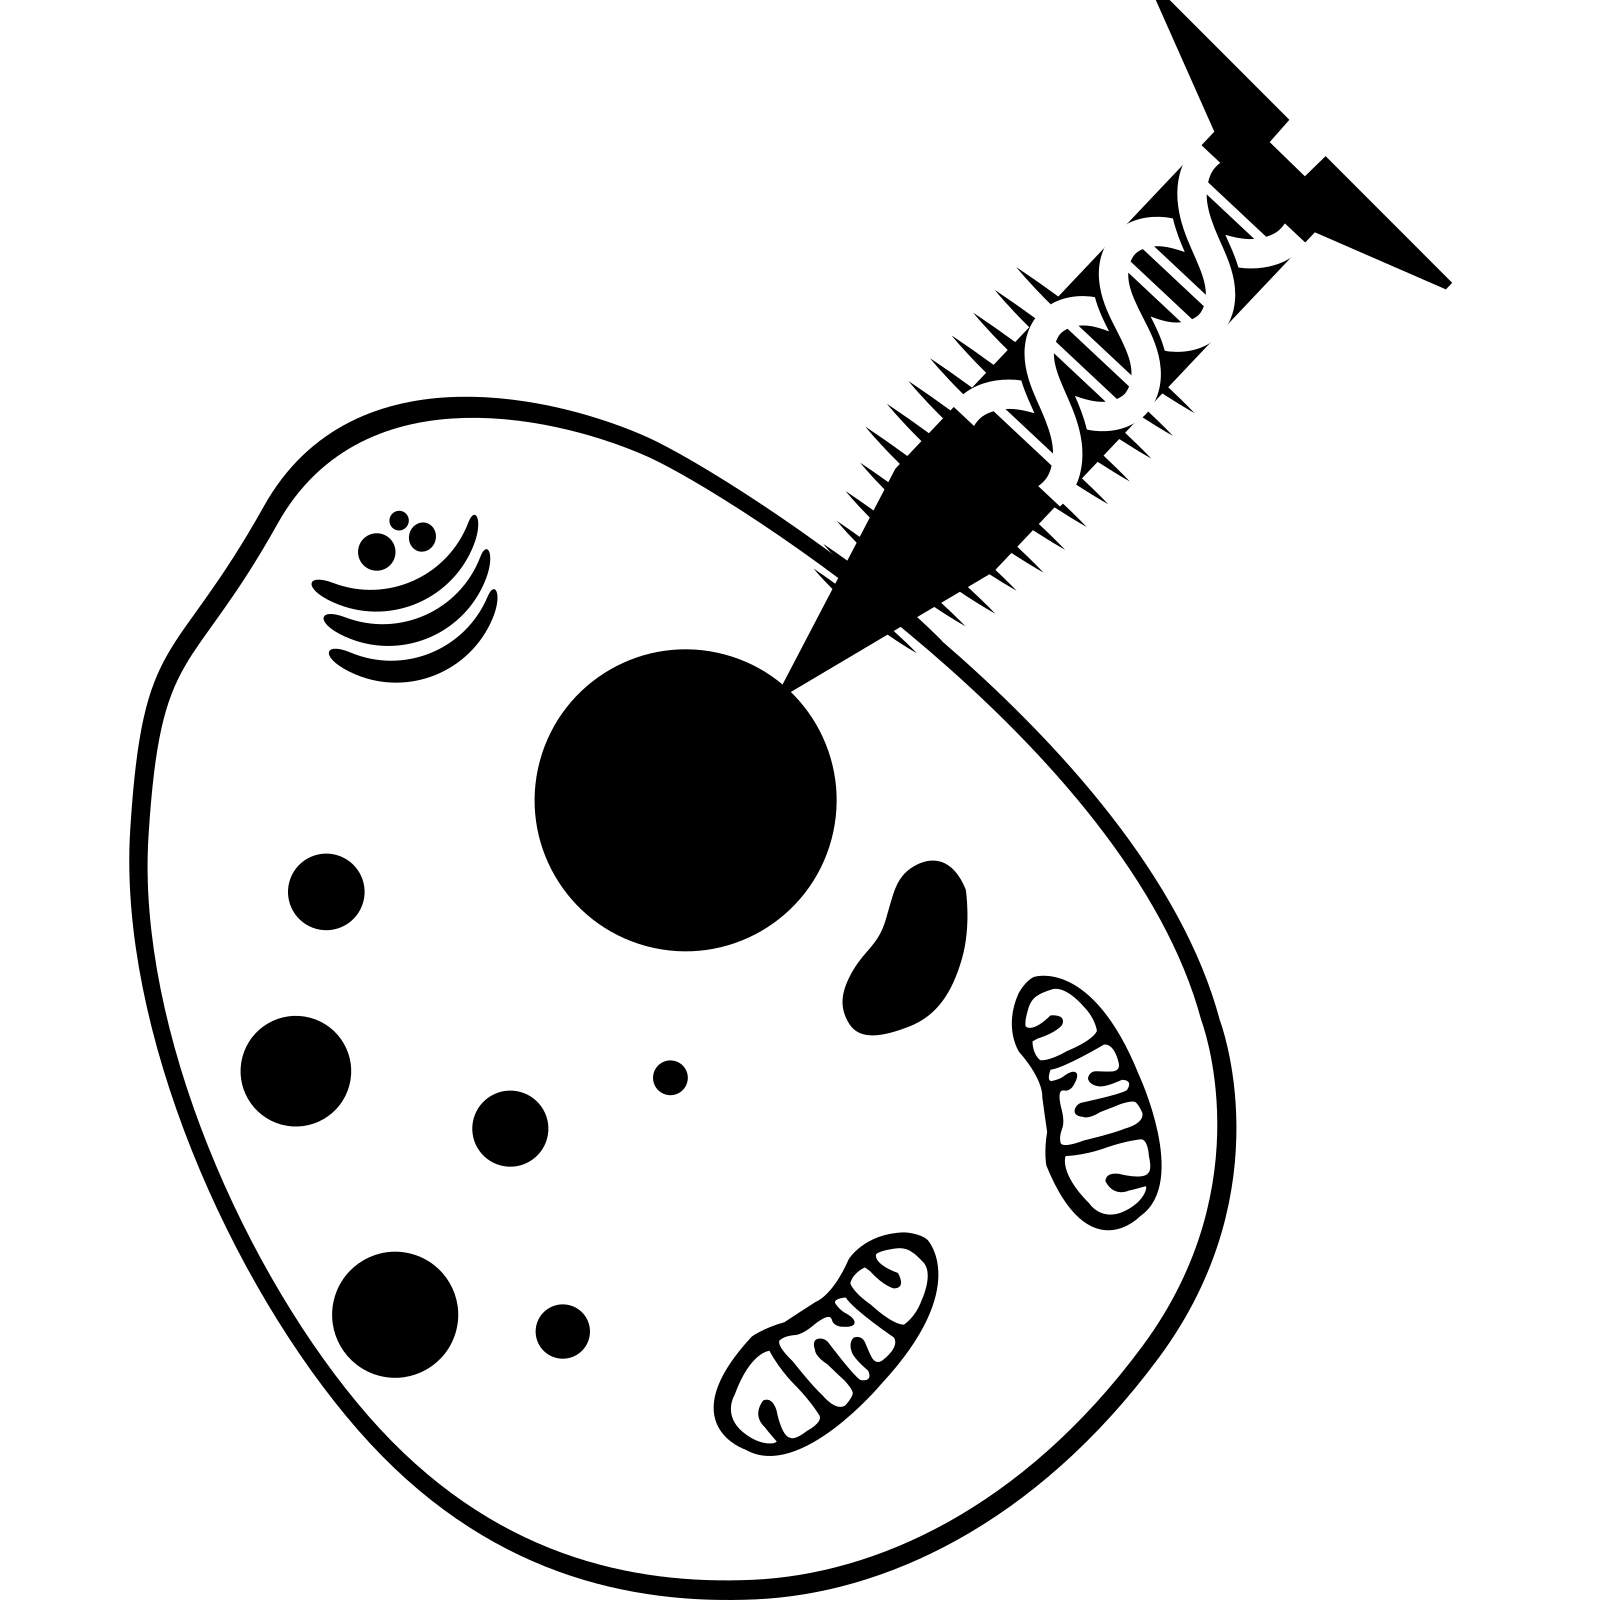
\includegraphics[width=0.2\textwidth]{figures/screw_logo_1600.png}
Screw aims to provide a series of CWL+Dockerised tools, mini-workflows and complete template workflows for creating fully reproducible SC-WGBS analyses.

\end{block}


\begin{block}{Reproducible Research with CWL and Docker}
Reproducible research means completely reproducing a given bioinformatic analysis
This requires having the exact \textbf{data}, \textbf{code} and \textbf{software} that was used.

\begin{itemize}
\item Open data in bioinformatics is a fairly solved problem.
\item Code is getting there with RMarkdown/Jupyter, but could be better.
\item Software versions (and accompanying OS/ecosystem) are a big problem.
\end{itemize}
\textbf{CWL} aims to solve the code problem by providing a uniform and fully reproducible way of representing bioinformatics workflows. \textbf{Docker} aims to solve the software version problem by providing the exact environment in which an analysis was run. Together, they promise to help bioinformaticians to publish fully reproducible research.

\textbf{Dockstore} enables easy sharing of workflow components to help build new, reproducible, workflows. 
\begin{figure}
\begin{center}
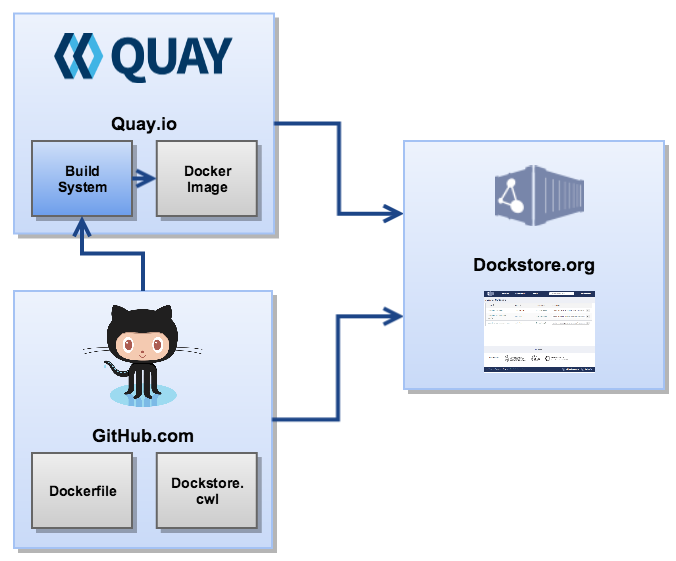
\includegraphics[width=0.9\textwidth]{figures/dockstore_logos.png}
\end{center}
\caption{\textbf{Docker, CWL and Dockstore.} CWL workflows (and Docker build files) are kept on GitHub. Quay.io automatically builds Docker images from these. Dockstore enables sharing of CWL-specified tools and workflows, along with a Docker image containing exact software. Image reused from dockstore.org under the Apache 2.0 license.}
\end{figure}
\end{block}





\begin{block}{What SC-WGBS Data Looks Like}
SC-WGBS data tends to have a reasonable number of cells ($~$100 in currently published data, up to thousands in data being generated now). It also tends to have a lot of dropout -- lateral coverage in each cell ranges from 1\% to 20\%.

\begin{figure}
\begin{center}
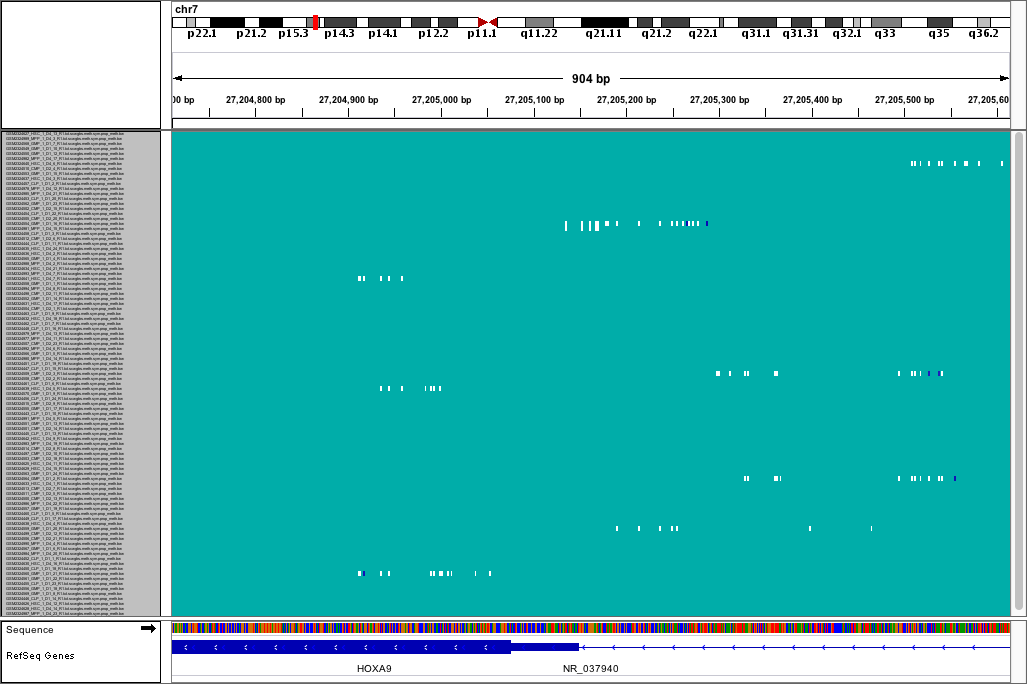
\includegraphics[width=0.9\textwidth]{figures/hoxa9_meth.png}

\end{center}
\caption{\textbf{DNA methylation around the \textit{HOXA9} TSS, from 100 single cells.}  Blue blocks indicate methylated CpGs, white unmethylated. Teal indicates missing data. DNA methylation data is very sparse -- only a handful of libraries have any coverage at all within a given window. Data from \cite{Farlik2016}; BigWIGS were generated by Screw and visualised in IGV.}
\end{figure}
\end{block}




\end{column}

%%%%%%%%%%%%%%%%%%%%%%%%%%%%%%%%%%%%%%%%%%%%%%%%%%%%%%%%%%%%%%%%%%%%%%%%%%%%%%%%%%%%
% COLUMN 2
%%%%%%%%%%%%%%%%%%%%%%%%%%%%%%%%%%%%%%%%%%%%%%%%%%%%%%%%%%%%%%%%%%%%%%%%%%%%%%%%%%%%

\begin{column}{.65\textwidth}
\vspace*{-\baselineskip}
  \begin{columns}[t,totalwidth=\textwidth]
    \begin{column}{.48\textwidth}
	%Second column, above figure
    
	
	\end{column}

	\begin{column}{.48\textwidth}
	%Third column, above figure
	
	\end{column}
  \end{columns}

	\begin{block}{Screw Workflow}
	\begin{center}
  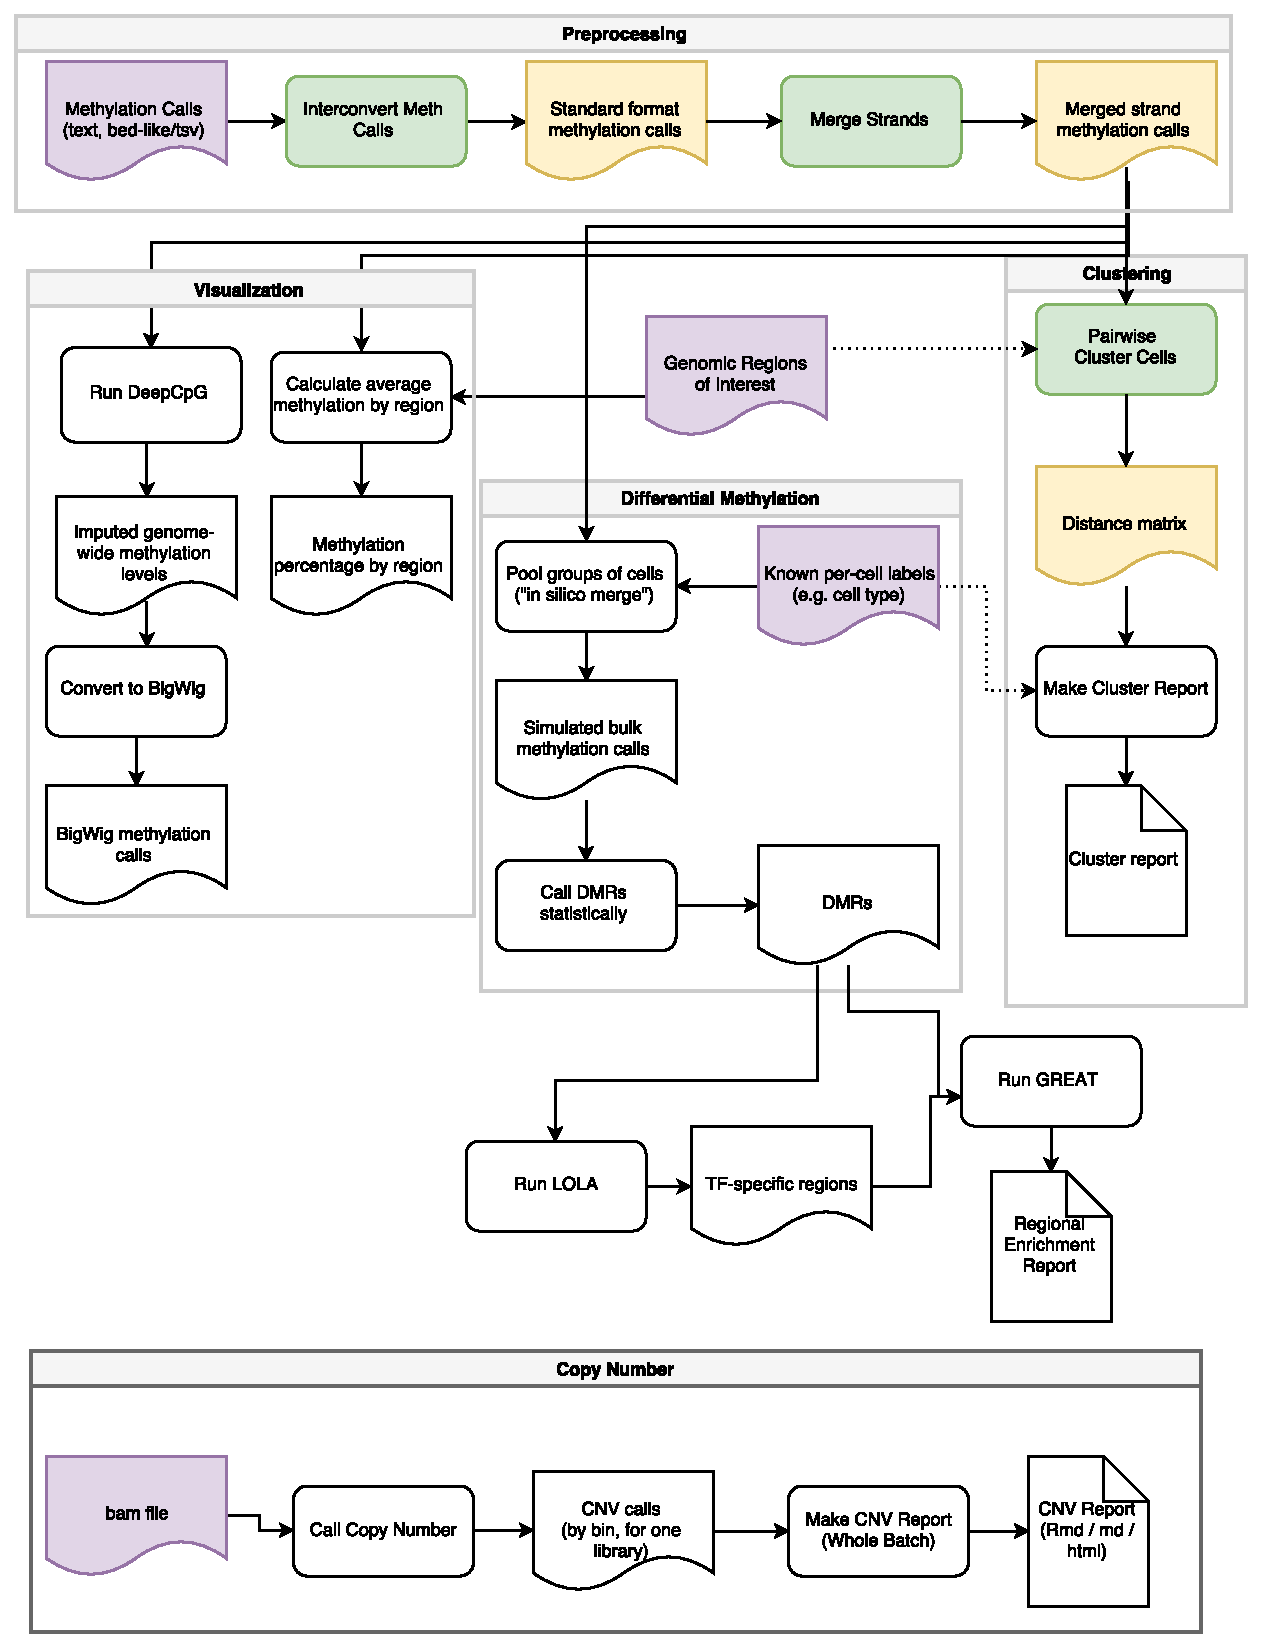
\includegraphics[width=0.95\textwidth]{figures/workflow_diagram.pdf}
  \end{center} 
  \end{block}
  \begin{columns}[t,totalwidth=\textwidth]


\begin{column}{.48\textwidth}
   

% Second column, below figure   
\begin{block}{Preprocessing: Format Interconversion}
	One of the challenges in DNA methylation is the lack of a standard data format. Neither BED nor WIG/BigWIG quite suit the requirements, so every data set uses its own custom BED-like format. Screw provides a script to convert from different formats into a format used internally by the rest of the Screw tools. We will add formats as we analyse existing public data sets. 
\begin{figure}
\begin{center}
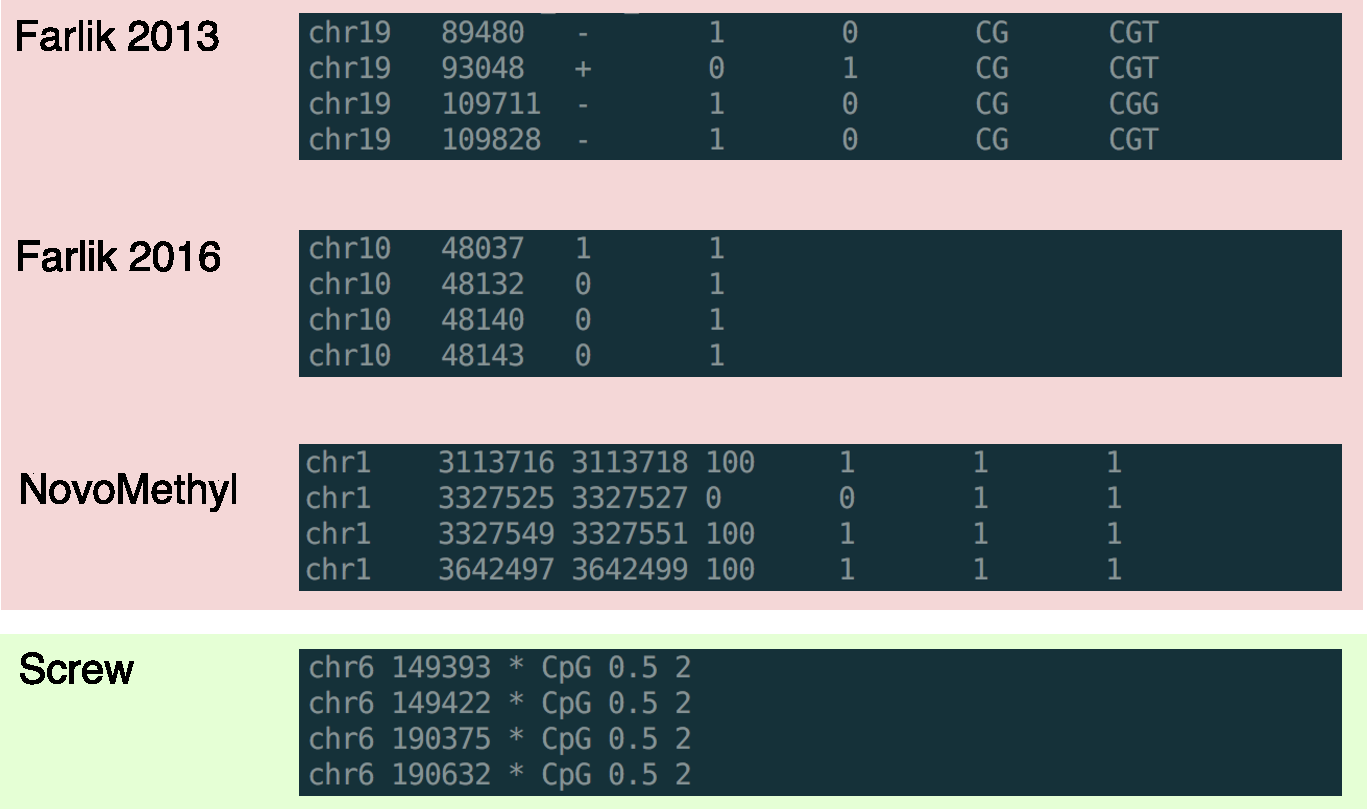
\includegraphics[width=0.9\textwidth]{figures/data_types.pdf}
\caption{\textbf{Diverse DNA methylation formats.} Formats from two published papers (\cite{Farlik2013} and \cite{Farlik2016}), NovoMethyl output format, and Screw's standard internal format.}
\end{center}
\end{figure}

\end{block}

\begin{block}{Clustering}
\begin{figure}
\begin{center}
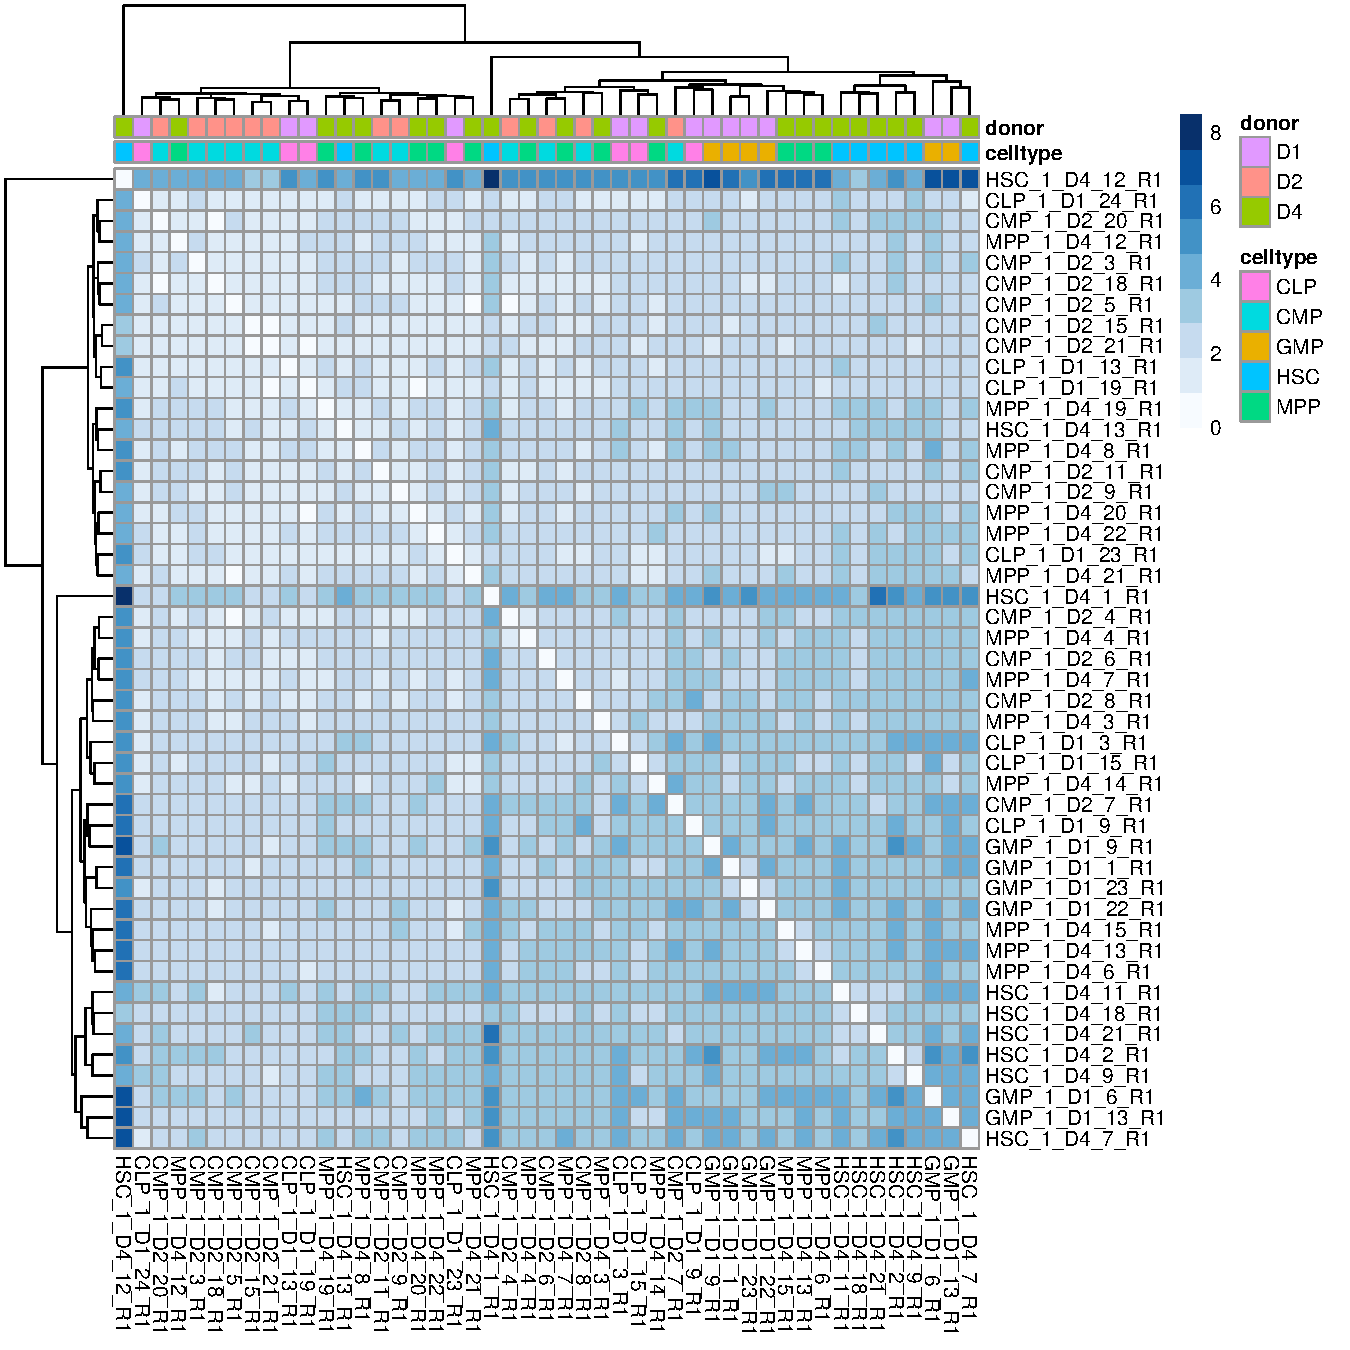
\includegraphics[width=0.8\textwidth]{figures/farlik_heatmap.pdf}
\caption{\textbf{Clustering of data from \cite{Farlik2016} using Screw.} A BED file containing locations of active enhancer sites in CD34+ bone marrow was used to filter the CpG sites. (Data from Enhancer Atlas.) Only 47/100 cells had coverage in those enhancer regions.  }
\end{center}
\end{figure}


\end{block}


\end{column}

	\begin{column}{.48\textwidth}
% Third column, below figure   

\begin{block}{CWL+Docker Technical Stumbling Blocks}
\begin{itemize}
\item CWL does not have a good way of processing a whole directory full of files, then passing them on to a single tool.
\item Quay.io maps tags to GitHub branches, but Docker treats tags like Git graph nodes, leading to problems refreshing branches while developing.
\item Our hyper-secure clinical IT environment won't let us use Docker, but will install Udocker, which CWL runner does not support (yet?)
\end{itemize}
\end{block}



\begin{block}{Future Work}
Many methods are currently being developed, and some have debuted in papers without (yet) an accompanying methods paper. In future we plan to include functionality for:
\begin{itemize}
\item tSNE plotting
\item Epiphylogenomics
\item DeepCpG
\item Other machine learning pipelines (e.g. from \cite{Farlik2016}) 
\end{itemize}

There are also around half a dozen SC-WGBS (or SC-RRBS) data sets published. We intend to use Screw to perform the first single cell DNA methylation meta-analysis. All code and data will be published in a fully-reproducible form. 

\end{block}


\begin{block}{Powered by hackathons and interns}
Development of Screw began at the NCBI Genomics Hackathon in March 2017, organised by Ben Busby. Since then, Chelsey Fang, a summer intern, has been working on the framework.


\begin{figure}
\begin{center}
  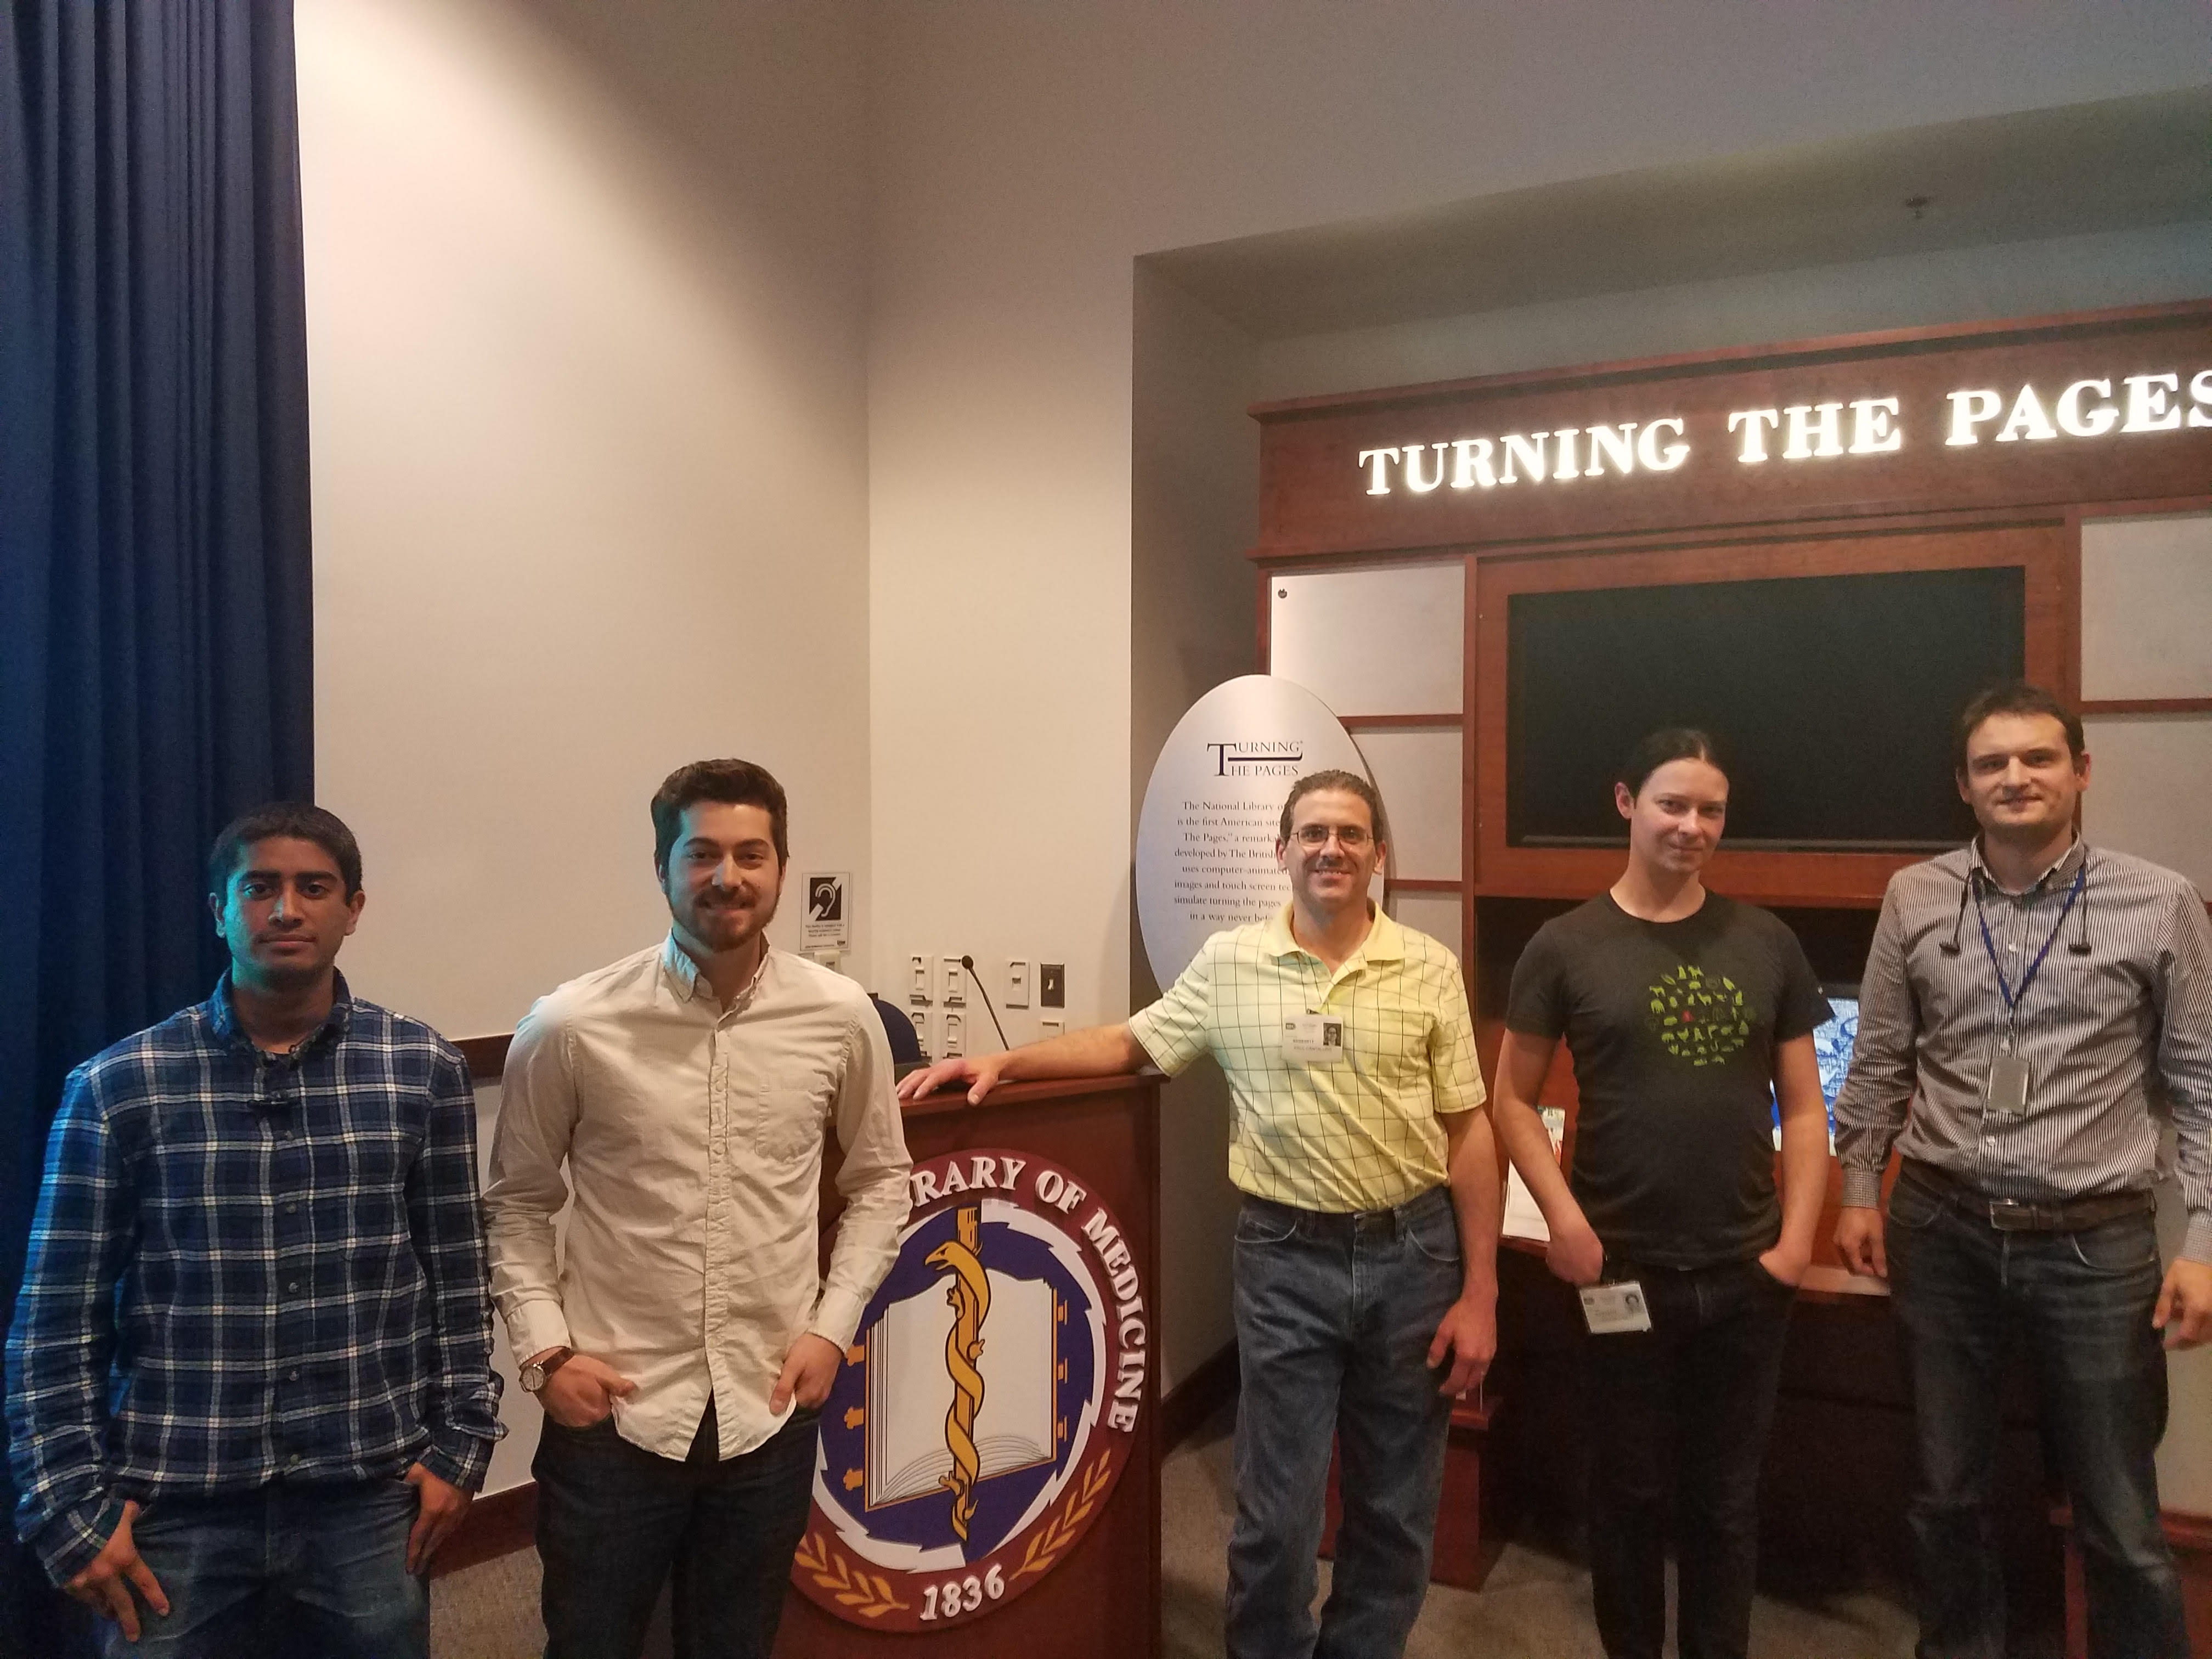
\includegraphics[width=0.7\textwidth]{figures/hackathon_team.jpg}
  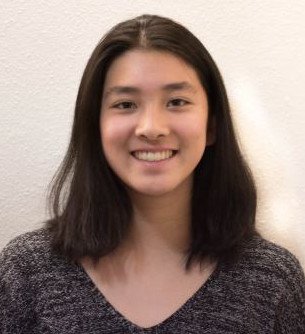
\includegraphics[width=0.2\textwidth]{figures/chelsey.jpg}
\end{center}
\caption{\textbf{The Screw team.} From left to right, Azhar Khandekar, Benjamin Decato, Paul Cantalupo (who worked in parallel on a similar project), Kieran O'Neill, Alexander Goncearenco; separate photo: Chelsey Fang.}
\end{figure}

\end{block}

\begin{block}{References}

\printbibliography[heading=none]
\end{block}



\begin{block}{Contact/GitHub}
\textbf{Code/examples:} \verb1https://github.com/Epigenomics-Screw1  

\textbf{Kieran O'Neill:} koneill@bcgsc.ca 

\end{block}
 
\end{column}

  \end{columns}
\end{column}


\end{columns}

\end{frame}

\end{document}
